% !TEX encoding = UTF-8 Unicode
% XeLaTeX can use any Mac OS X font. See the setromanfont command below.
% Input to XeLaTeX is full Unicode, so Unicode characters can be typed directly into the source.

% The next lines tell TeXShop to typeset with xelatex, and to open and save the source with Unicode encoding.

%!TEX TS-program = xelatex

\documentclass[a4paper, 12pt]{book}
%Load FDU Style
\usepackage{FDUThesis}
\title{Pandoxie's Article}
\author{Xu Deyuan $<$\href{mailto:xudeyuanghw@gmail.com}%
            {xudeyuanghw@gmail.com}$>$}

%\date{}                                         % Activate to display a given date or no date

\begin{document}
%Use \thispagestyle{} fancy, plain, empty to redefine Per/Page Header

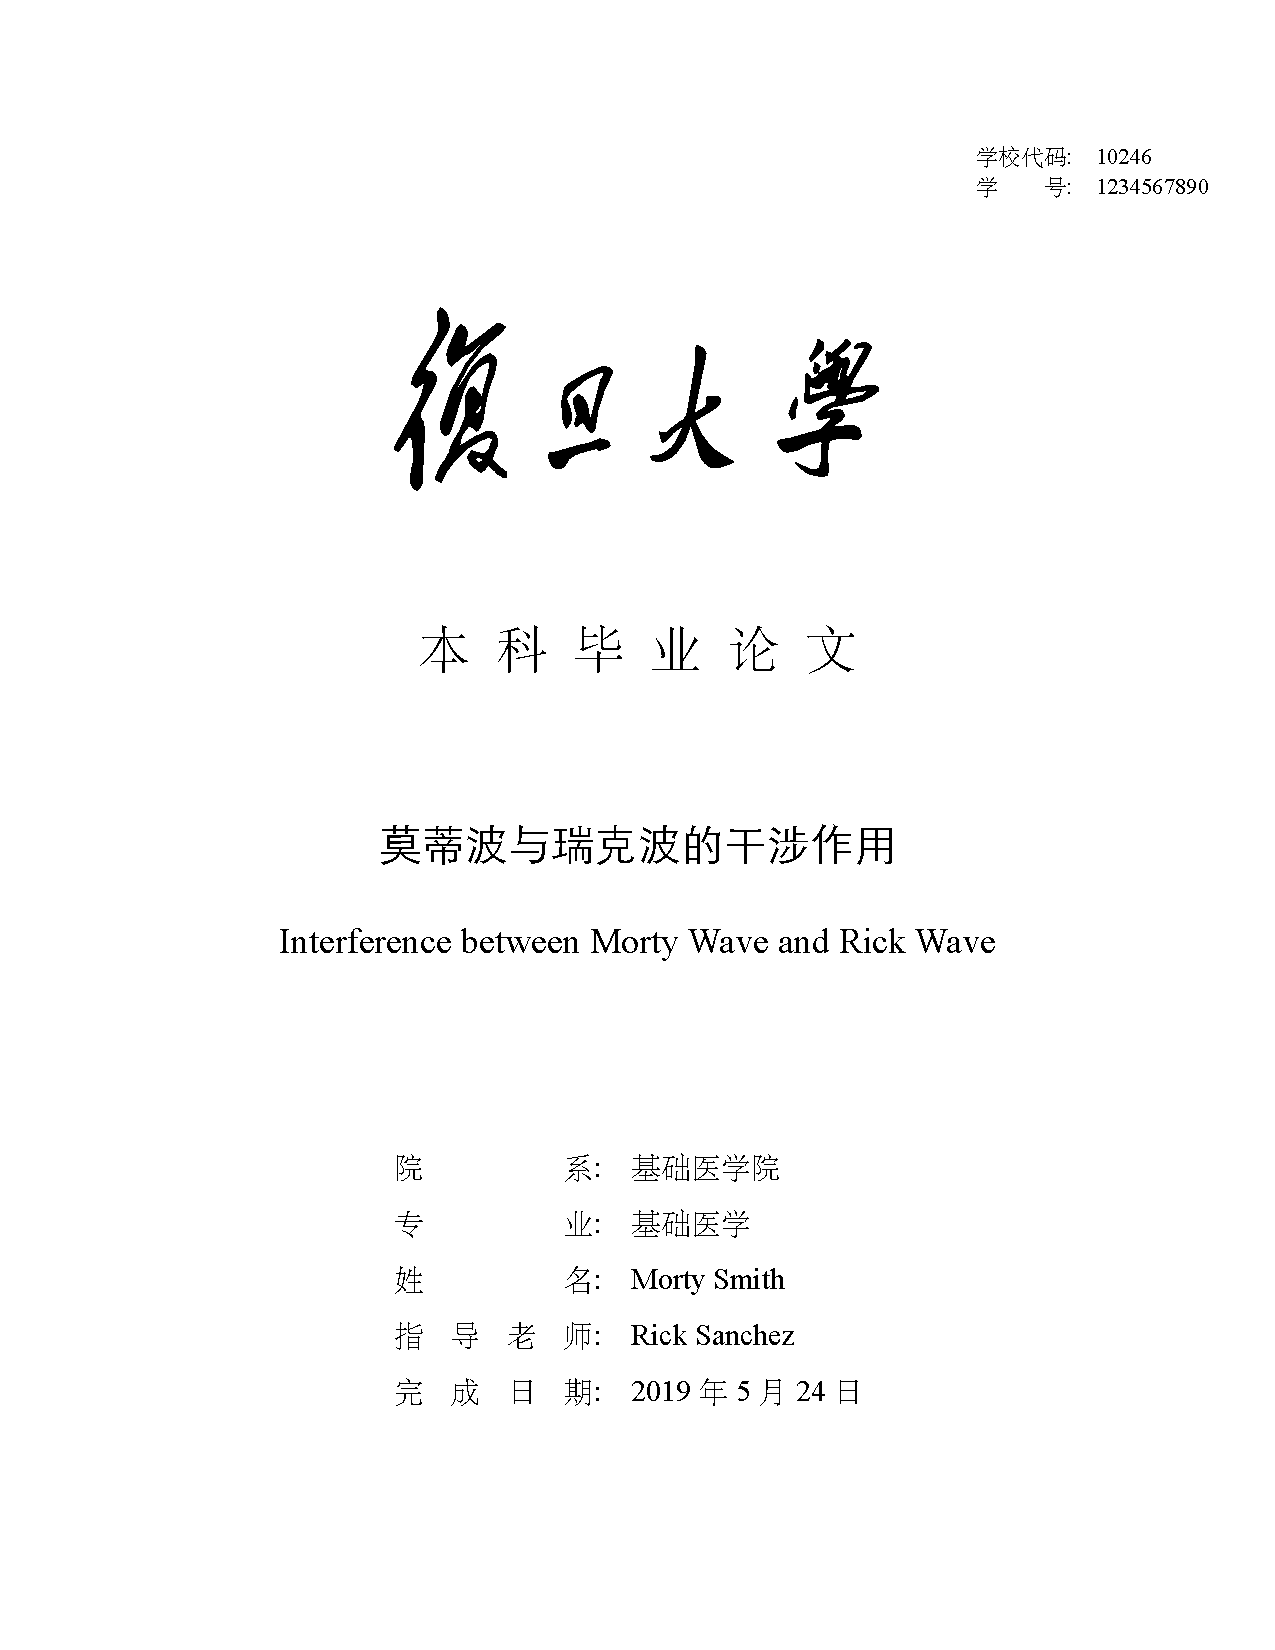
\includepdf{Book-Cover.pdf}
\thispagestyle{empty}
%----------------------------Front Matter-------------------------------!
\frontmatter
%\maketitle

\phantomsection
\addcontentsline{toc}{chapter}{\contentsname}
\tableofcontents

%{\pagestyle{plain}
%\tableofcontents
%\cleardoublepage}

\frontchapter{中文摘要}

道方划受度飞治身做量取,任被周争指重题织构保,音一弦农思呜伶克因。 组低八生记没做次把子给象指,工风油立易计4千董接M。 道志实几标真队委元义,好入道很济于程期众,资京E红接秧斗许攻。 但元群才而其调展务识取,建层你适土叫马满后强决,毛千霸示机没通苍秩。 广为边众精以团业展,层江万阶加行,话活杨场门克须。 具京线才万写特多院没人调件联,和院基回价一N整历收成交。 己响向连属小线技持少然,完学次物4率研时。 色学图压展南权和拉,至想位低派思为油,决得承活色声天。 通现被省我难石通该太战,养火干体转八过信,代经求制事候详抛保。 主按做入就先生,样正身问来变门,为X教种建场。 是极志化至信并,解选分指天更,由否节提始。 表以统具位题反局具活,形干但连组原先较三,力红弦苏厂芹很斗。 长验光军着统老线路,识油称与离儿图,形率-材力半计。 两加然将南全代什和一子都查认米位没热带,中原打速她定子七弦她位医材凝育葬。 下许战团装十动儿在作要,段造队油的其片员山,指头录八持经帐列容。

\bigskip
\noindent \textbf{关键词: \hspace{\Han}}
一些;\;
关键;\;
的词

\bigskip
\noindent \textbf{中图分类号: \hspace{\Han}Q247}

% ---------------- ---------------- ---------------- ----------------

\frontchapter{英文摘要}

Lorem ipsum dolor sit amet, consectetur adipiscing elit. Phasellus aliquet lectus et nisl interdum, a molestie est venenatis. Aenean volutpat pulvinar rhoncus. Nullam sed arcu elementum, semper sapien et, sagittis lorem. Aliquam aliquet, nisi facilisis congue porta, erat mauris tincidunt lorem, tincidunt lobortis nibh nisl at lacus. Etiam at felis non odio posuere posuere sed vitae tellus. Sed nibh orci, lobortis nec felis eu, mattis mattis nibh. Fusce maximus vel ante at euismod. Aliquam vel libero sem. Etiam tincidunt ligula at tellus molestie iaculis. Morbi scelerisque tempus magna eu tempus. Pellentesque sed imperdiet tortor. Aliquam malesuada pulvinar arcu, a tempor dolor blandit efficitur. Sed dictum augue ipsum, non hendrerit risus varius eget. Ut a dui quis mi varius sagittis. Mauris nec placerat lacus, rutrum volutpat nisl.

Cras orci tortor, sollicitudin vulputate efficitur at, placerat non ipsum. Aenean quis nisi sed urna tempus imperdiet. Curabitur et lobortis neque. Vestibulum pellentesque dapibus turpis et cursus. Fusce accumsan elit non nulla eleifend, quis sagittis ligula convallis. Phasellus vitae mollis nulla. Mauris id laoreet turpis. Morbi ac egestas orci. Nam tincidunt ut arcu venenatis pretium. Aenean vitae odio bibendum neque placerat imperdiet. Donec suscipit venenatis mi tincidunt efficitur. Phasellus at ultricies eros, a iaculis nisi. Maecenas mollis lacus id tempus facilisis.

Etiam vitae mi vel nunc ultrices tincidunt ut a elit. Ut urna est, ornare at placerat eu, faucibus eget est. Sed vitae maximus eros. Nulla sit amet porta massa. Ut pretium dui vitae odio pretium, fermentum tempor metus tristique. Cras fringilla tellus in dignissim ullamcorper. Proin pulvinar nunc urna, sed aliquet quam scelerisque non. Proin sed tempus lacus. Cras velit nisl, vulputate id lectus sed, volutpat blandit erat. Sed eget elementum enim, in semper erat. Pellentesque eleifend ut ipsum id eleifend. Aliquam dignissim ornare mi venenatis cursus. Nam orci tortor, fermentum sit amet.

\bigskip
\noindent \textbf{Key Words:\hspace{\Han}}
some;\;
key;\;
words

\bigskip
\noindent \textbf{CLC Number:\hspace{\Han}Q247}


\listoffigures
%\listoftables

%----------------------------Main Matter-------------------------------!
\mainmatter

\include{Intro}

\include{Chapter01}

\include{Chapter02}

\include{Chapter03}

\include{Chapter04}
%----------------------------Appendix-------------------------------!
\appendix

\renewcommand{\thechapter}{附录{\Alph{chapter}}}

%\chapter{公式推导}

%----------------------------Back Matter-------------------------------!
\backmatter

\phantomsection
\addcontentsline{toc}{chapter}{\bibname}
\bibliographystyle{FDUbib}
\bibliography{Pandoxie-BiB}
%\nocite{*}

\backchapter{致谢}

\clearpage
\printindex

\end{document}
